%(BEGIN_QUESTION)
% Copyright 2009, Tony R. Kuphaldt, released under the Creative Commons Attribution License (v 1.0)
% This means you may do almost anything with this work of mine, so long as you give me proper credit

Pure nitrogen (N$_{2}$) gas is often used as an {\it inerting} agent to displace air from the vapor space of tanks holding some chemically reactive liquid(s) such as flammable fuels.  Nitrogen is quite un-reactive at ambient temperatures, and so a ``blanket'' of this gas will do an effective job isolating liquid substances from contact with air in a tank:

$$\includegraphics[width=15.5cm]{i04119x01.eps}$$

Suppose exactly 45 kilograms of liquid nitrogen are vaporized to form nitrogen gas at atmospheric pressure and a temperature of 20 $^{o}$C for the purpose of ``blanketing'' a fuel storage tank made of mild steel.  How much air volume will this much nitrogen displace, in units of liters and also cubic feet? 

\vskip 20pt \vbox{\hrule \hbox{\strut \vrule{} {\bf Suggestions for Socratic discussion} \vrule} \hrule}

\begin{itemize}
\item{} Explain the purpose served by the pressure regulating valve on the nitrogen supply line to the tank.
\item{} Explain the purpose of the special ``PSV'' valve located on the roof of the tank.
\item{} Based on what you know about the N$_{2}$ molecule, explain why nitrogen gas is so un-reactive at low temperatures.
\item{} Will more or less mass of nitrogen be required to ``blanket'' a fuel storage tank if the ambient temperature falls (assuming an unchanged liquid volume inside the tank)?
\item{} Based on what you know of nitrogen's chemical properties, does it constitute a health or safety hazard?  Why or why not?
\item{} Suppose this blanketing system were functioning on a very cold winter day.  Would this environmental change affect your calculation of displaced air volume?  Explain why or why not.
\item{} Could a nitrogen blanketing system such as this affect the measurement accuracy of a level transmitter installed in this tank?  Explain why or why not.
\end{itemize}

\underbar{file i04119}
%(END_QUESTION)





%(BEGIN_ANSWER)

$V$ = 38,680 liters

%(END_ANSWER)





%(BEGIN_NOTES)

Nitrogen gas (N$_{2}$ molecules) have a molecular weight of approximately 28 grams per mole.  Therefore:

$$\left({ 45 \hbox{ kg} \over 1}\right) \left({1000 \hbox{ g} \over 1 \hbox{ kg}}\right) \left( {1 \hbox{ mol N}_2 \over 28 \hbox{ g}} \right) = 1607.14 \hbox{ moles of N}_2 \hbox{ gas}$$

We may now use the Ideal Gas Law to solve for the volume of this nitrogen gas at 20 $^{o}$C (293.15 K):

$$PV = nRT$$

$$V = {nRT \over P} = {(1607.14 \hbox{ mol}) (0.0821 \hbox{ l-atm/mol-K}) (293.15 \hbox{ K}) \over 1 \hbox{ atm}} = 38680 \hbox{ liters}$$

This figure may be then unit-converted into cubic feet:

\vskip 10pt

$$\left(38680 \hbox{ l} \over 1 \right) \left(1000 \hbox{ cm}^3 \over 1 \hbox{ l}\right) \left(1^3 \hbox{ in}^3 \over 2.54^3 \hbox{ cm}^3\right) \left(1^3 \hbox{ ft}^3 \over 12^3 \hbox{ in}^3\right) = 1365.97 \hbox{ ft}^3$$

\vskip 10pt

The tank's material (mild steel) is extraneous information, included for the purpose of challenging students to identify whether or not information is relevant to solving a particular problem.

%INDEX% Chemistry, stoichiometry: moles
%INDEX% Process: nitrogen inerting ``blanket'' for storage tank

%(END_NOTES)


